\section{Emmagatzematge Extern}

Les solucions de backup facilitades no s'adeqüen a les necessitats del projecte. S'han plantejat els diferents escenaris i s'ha conclòs que el temps de recuperació del servei és massa alt en qualsevol de les propostes. En conseqüència s'ha desenvolupat una solució alternativa que permeti una alta seguretat i disponibilitat de les dades. 

La criticitat de les dades del projecte es troba en les dades de les cabines de discs. És per això que proposem la creació d'un segon CPD que contingui la informació del sistema d'emmagatzematge del CPD principal, de forma que les dades estiguin replicades en temps real i sempre disponibles. Existirà un període de consistència eventual mínim inevitable degut al temps de propagació dels canvis. El gran avantage d'aquest sistema es que en cas que la capa de storage principal esdevingués inoperativa, els servidors de la capa de Frontals utilitzarien el storage auxiliar com a "backend".

Aquesta solució és assumible en aquest projecte gràcies al tipus d'aplicació que s'hi allotja. El nombre de escriptures serà molt baix, per tant, la replicació de les dades no serà extramadement costosa. També cal tenir en compte que l'arquitectura de la plataforma està pensada per fer "caching". És a dir, que s'intenta accedir a la capa d'emmagatzemage el menys possible. 

Les característiques tècniques de l'emmagatzematge auxiliar seran inferiors que les de producció. Caldrà que el tamany del "working set" de dades sigui equivalent, però la velocitat d'accés serà inferior donat que no será un punt crític per al aprovisonament del servei. 

D'altre banda, la resta de màquines es troben redundades, per tant, la resta de màquines no disposen d'informació no volàtil. Certament hi ha informació especifica de cada tipus de màquina, com configuracions. No obstant, es poden utilitzar solucions de desplegament de màquines mitjançant orquestració.

\begin{figure}[H]
    \centering
    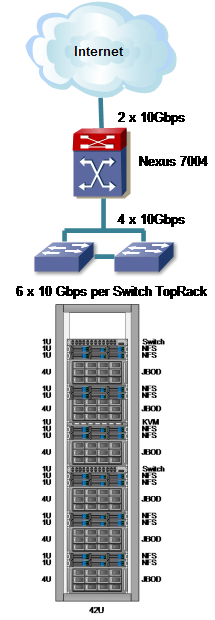
\includegraphics[height=0.55\textwidth]{cpdbackupnetwork}
    \caption{Arquitectura Centre de Dades de Backup \label{fig:CPDbackup}}    
\end{figure}

El collocation center proposat per allotjar aquest CPD serà el ofert per la empresa CPDs Céspedes S.L.. Tot i que CPD Céspedes proporciona menys fiabilitat (una certificació d’un 99,671\% d'uptime) i una menor eficiència energètica (amb un PUE més alt que la resta).

Es descarten els seus competidors, el Mordor Colocation Center, on s’allotja el CPD principal que en cas de catàstrofe o d’incendi es podria veure malmesa tota la informació i no podríem mantenir una de les parts mes importants del negoci, la informació d’usuari. L’altre competidor, Modular Containers S.A. només ofereix un allotjament per 19 racks, per tant, per allotjar els docs racks necessaris de l’arquitectura hauríem de suportar el cost de l’espai de 19 racks, cosa que el fa un malbaratament innecessari.

En quant a maquinari, tal i com podem veure a la figura anterior, no hi ha replicació dels elements de xarxa i disposa d’una connexió a internet de 20Gbps, per els motius anteriorment descrits no te la necessitat de duplicar els elements donat que l’objectiu d’aquest CPD és mantenir una còpia de les dades en temps real i fàcilment accessible.

Per últim, s'ha tingut en compte el desdoblament del CPD principal com a possibilitat a l'hora de distribuir la informació i aconseguir un servei amb una disponibilitat més alta (de forma que si cau un CPD, un altre pogués continuar donant servei encarà que suposés un degradament del servei) però s'ha descartat pels inconvenients que pot tenir aquest sistema a l'hora de mantenir-ho. Aquesta configuració suposava un increment al voltant dels 2M\euro  sobre el pressupost d'aquest projecte superant així el pressupost establert.